\documentclass[10pt, xcolor=table]{beamer}
%\usetheme{Boadilla}
%\usecolortheme{beaver}
%\usepackage[latin1]{inputenc}
%\useoutertheme{split}
\setbeamertemplate{navigation symbols}{}
\usefonttheme[onlymath]{serif}
\usepackage[export]{adjustbox}
\usepackage{amsmath}%
%\usepackage[table]{xcolor}
\usepackage{amsthm}%
\usepackage{amsfonts}%
\usepackage{amssymb}%
\usepackage[algo2e]{algorithm2e}
\usepackage{algorithmic}  
\usepackage{algorithm}
\usepackage{tikz}
\usepackage[english]{babel}
\usepackage{amsmath, amssymb}
\usepackage{verbatim}
\usepackage{mathrsfs}
%\usepackage{epstopdf}
\usepackage{graphicx}
%\mode<presentation>
%{
%	\usetheme{CambridgeUS}
%	\usecolortheme{dolphin}
%	\usecolortheme{rose}
%	\setbeamercovered{transparent}
%}
\newcommand{\mrel}{\mathrel{\bigcirc}}
%\usepackage[onehalfspacing]{setspace}
%\setbeamertemplate{footline}[frame number]
\DeclareMathOperator*{\Bigcdot}{\scalerel*{\cdot}{\bigodot}}
% Macros
\def\a{\alpha} \def\b{\beta} \def\c{\gamma} \def\d{\delta} \def\r{\rho}
\def\e{\epsilon} \def\ve{\varebsilon} \def\k{\kappa} \def\p{\pi} \def\th{\theta}
\def\l{\lambda} \def\m{\mu} \def\s{\sigma} \def\t{\tau} \def\w{\omega} \def\z{\zeta}
\def\D{\Delta} \def\G{\Gamma} \def\W{\Omega} \def\P{\Phi} \def\L{\Lambda}
\def\bdm{\begin{displaymath}} \def\edm{\end{displaymath}}
\def\bni{\begin{itemize}} \def\ei{\end{itemize}}
\def\bnen{\begin{enumerate}} \def\een{\end{enumerate}}
\def\fa{\forall}
\def\be{\begin{equation}} \def\ee{\end{equation}}
\def\fn{\footnote} \def\bn{\begin} \def\nit{\noindent}
\def\iff{\textit{~if and only if~~}}
\renewcommand*{\thefootnote}{\fnsymbol{footnote}}
% THEOREMS -------------------------------------------------------
\newtheorem{thm}{Theorem}%[section]
\newtheorem{cor}[thm]{Corollary}
\newtheorem{lem}[thm]{Lemma}
\newtheorem{prop}[thm]{Proposition}
\newtheorem{claim}{Claim}
\theoremstyle{definition}
%\newtheorem{defn}[thm]{Definition}
\theoremstyle{remark}
\newtheorem{rem}[thm]{Remark}
%%\numberwithin{equation}{section}  
 
\newcommand{\N}{\mathbb{N}}
\newcommand{\Z}{\mathbb{Z}}
\newcommand{\R}{\mathbb{R}}
\newcommand{\ls}{\left\{}
\newcommand{\rs}{\right\}}


\title[Interaction-Partitioned Topic Model (IPTM)]{ \vspace{-.25cm} \\ A Network Model for \\Dynamic Textual Communications \\with Application to
	Government Email Corpora}
\author[\quad B. Kim, A. Schein, B. Desmarais and H. Wallach\quad]{
Bomin Kim\textsuperscript{1}\and
\quad Aaron Schein\textsuperscript{3}\and\\
		Bruce Desmarais \textsuperscript{1}\and Hanna Wallach\textsuperscript{2,3}}
\institute{\textsuperscript{1} The Pennsylvania State University \and \textsuperscript{2} Microsoft Research NYC \and \textsuperscript{3} University of Massachusetts Amherst}


\newenvironment{changemargin}[2]{%
  \begin{list}{}{%
    \setlength{\topsep}{0pt}%
    \setlength{\leftmargin}{#1}%
    \setlength{\rightmargin}{#2}%
    \setlength{\listparindent}{\parindent}%
    \setlength{\itemindent}{\parindent}%
    \setlength{\parsep}{\parskip}%
  }%
  \item[]}{\end{list}} 

\begin{document}
 
\begin{frame}
  \titlepage
  \begin{center}
   \begin{tabular}{cc}
\hspace*{-.2in} \tiny \begin{minipage}{3.5in}
Work supported by NSF grants SES-1558661, SES-1619644, SES-1637089, and CISE-1320219)\\ ~\\~\\~\\~\\
\end{minipage}
& \includegraphics[scale=.05]{figures/NSF_logo.png}
\end{tabular}
\end{center}
\end{frame}




\begin{frame}{Motivation}
\Large
\begin{itemize}
\item Ties attributed with text
\begin{itemize}
\item International treaties
\item Legislative cosponsorship
\item Discussion networks on social media
\end{itemize}

\begin{center}
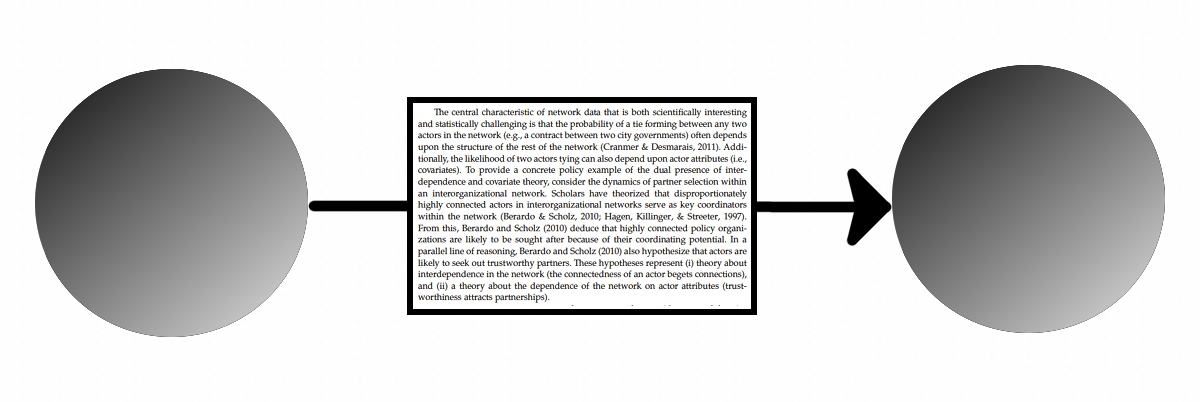
\includegraphics[scale=.2]{figures/tieWords}
\end{center} \vspace{-.1cm}
\item Network models can't model text
\vspace{.3cm}
\item Models for text...
\begin{itemize}
\item not designed for networks
\item simplistic network structure
\end{itemize}
\end{itemize}
\end{frame}

\begin{frame}{Interaction-Partitioned Topic Model (IPTM)}
\large
	\bni
	\item Probablistic model for time-stamped textual communications 
	\vspace{0.2cm}
	\item Integration of two generative models:
	\begin{itemize}
	 \item Latent Dirichlet allocation (LDA) for topic-based contents
	  \item Dynamic exponential random graph model (ERGM) for ties 
	  \end{itemize}
	\ei
		\vspace{0.4cm}
\centering \large\textit{``who communicates with whom about what, and when?"}
\end{frame}

\begin{frame}{Content generating process: LDA (Blei et al., 2003)}
\bni 
\begin{minipage}{0.7\linewidth}
\item For each topic $k =1,...,K:$\vspace{0.2cm}
	\begin{itemize}
		\item[1.] Choose a topic-word distribution over the word types\vspace{0.2cm}
		\item[2.] Choose a topic-interaction pattern assignment			
		\end{itemize}
		\vspace{0.2cm}
	\end{minipage}
	\begin{minipage}{0.25\linewidth}
			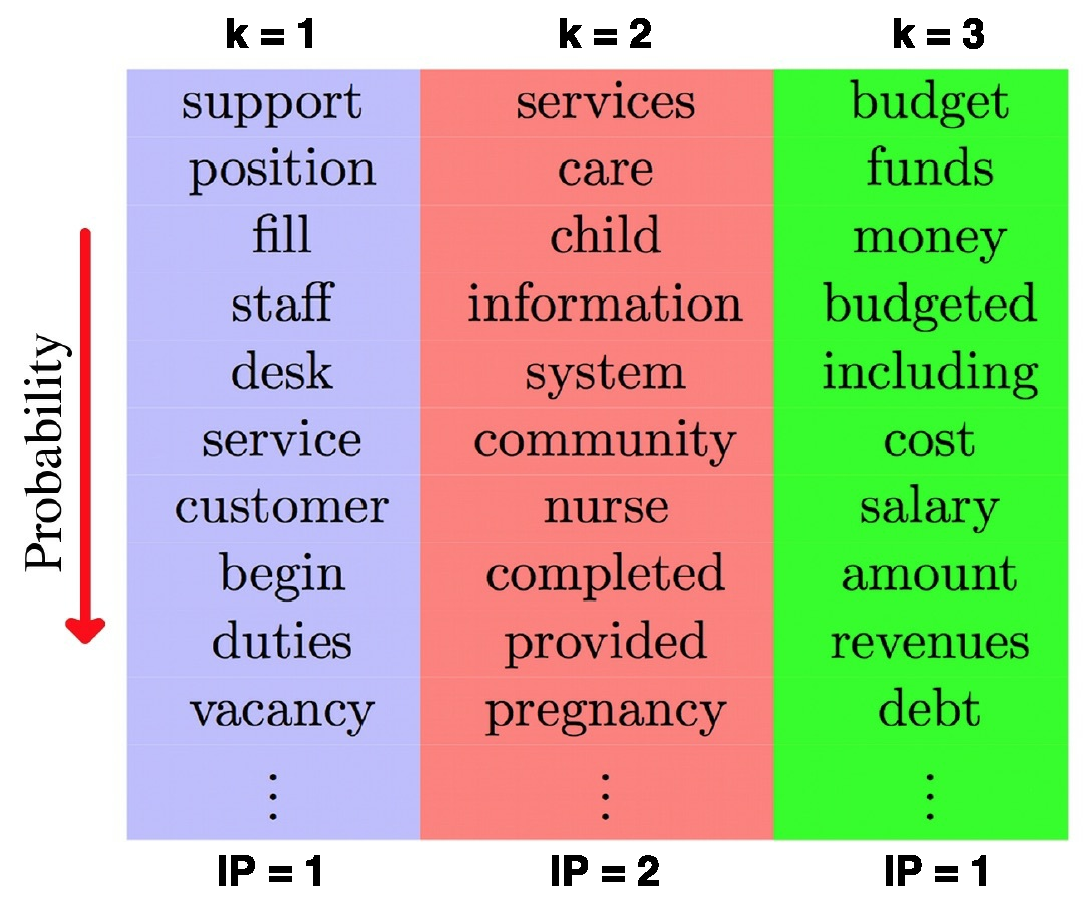
\includegraphics[width=1\textwidth]{figures/word.pdf}
				\vspace{0.2cm}
		\end{minipage}
			\begin{minipage}{0.68\linewidth}
				\item For each document $d =1,...,D:$ \vspace{0.2cm}
		\begin{itemize}
					\item[3-1.] Choose a document-topic distribution \\\vspace{0.1cm} 
		\item[3-2.] For each word in a document $n=1$ to $N^{(d)}$:\vspace{0.1cm} 
		\begin{itemize}
			\item[(a)] Choose a topic from document-topic distribution\vspace{0.2cm} 
			\item[(b)] Choose a word from topic-word distribution
		\end{itemize} 
			\end{itemize}
		\end{minipage}
		\begin{minipage}{0.3\linewidth}
	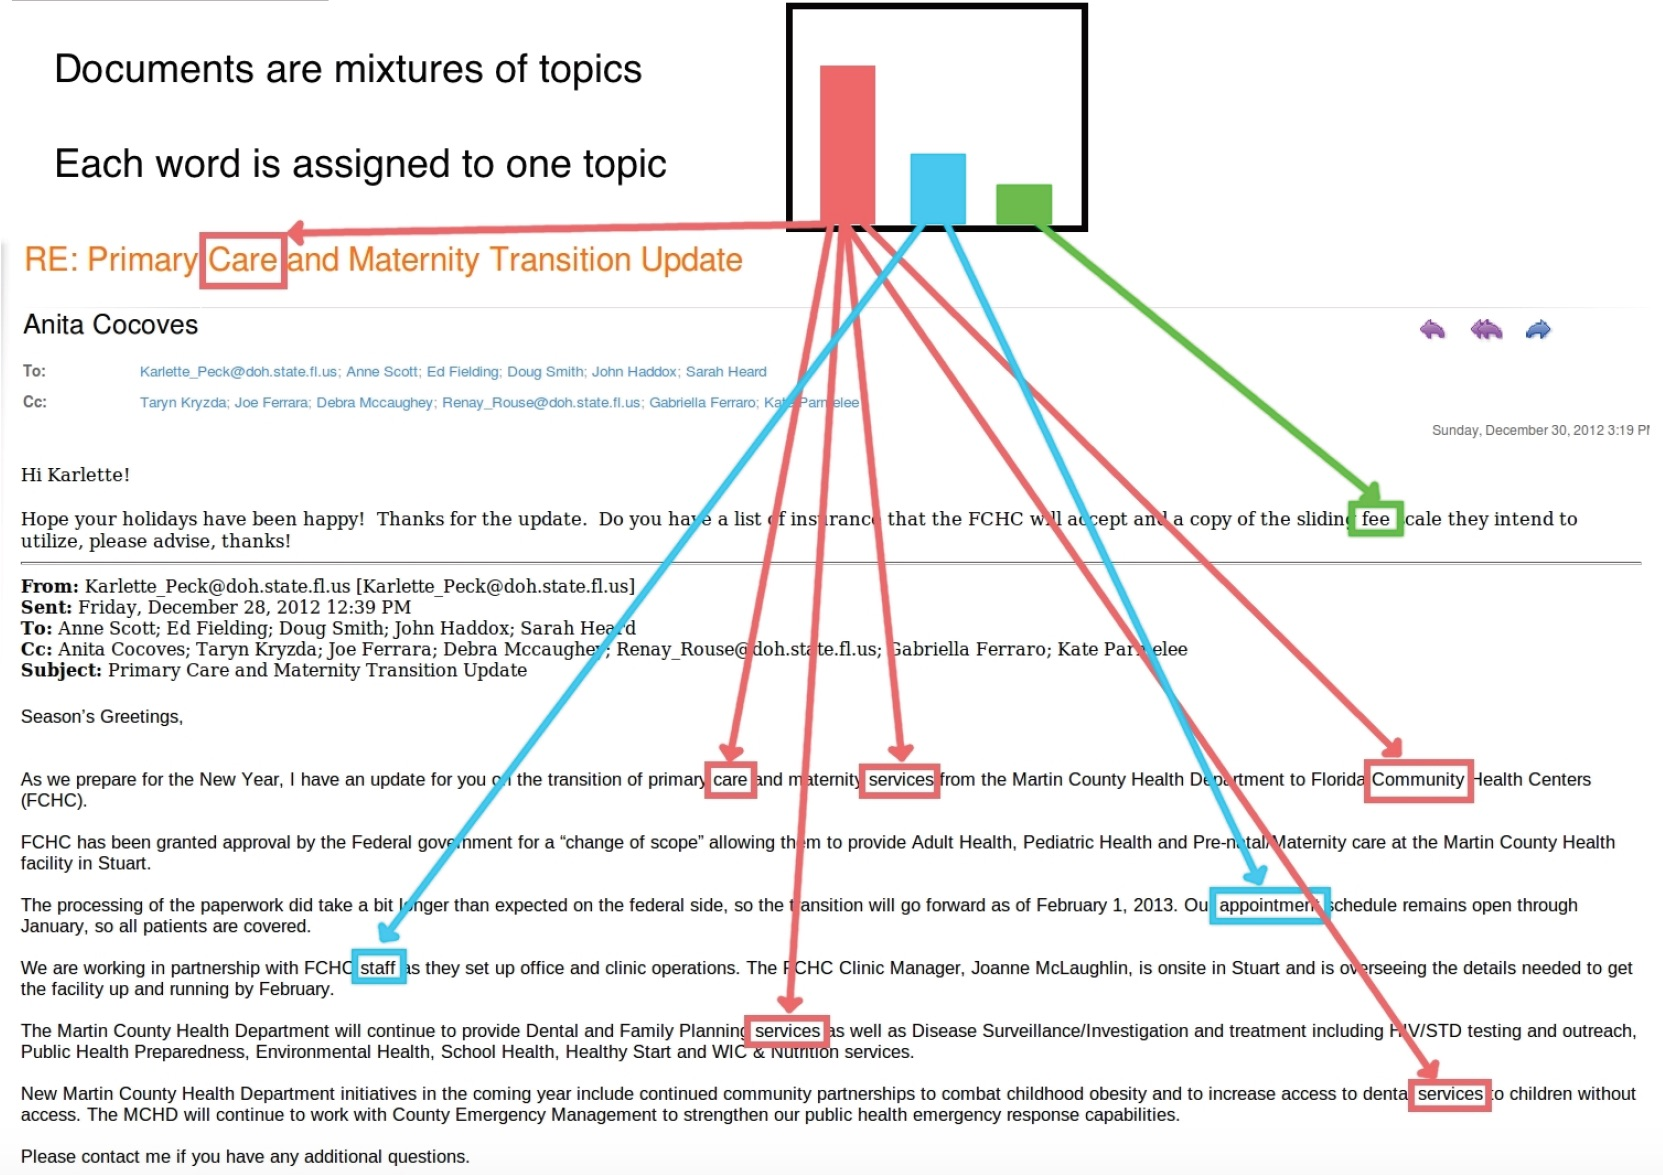
\includegraphics[width=1.05\textwidth]{figures/LDAimage.jpeg}
		\end{minipage}
		\vspace{0.2cm}
				\begin{itemize}\item[3-3] Calculate the distribution of interaction patterns within a document:
		 \footnotesize\begin{equation*}
		p_c^{(d)} = \Big({\sum\limits_{k: c_k=c} N^{(k|d)}}\Big)/{N^{(d)}},
		\end{equation*}\normalsize
	\end{itemize}
\ei	
\end{frame}


\begin{frame}{Network model components}
\large
\begin{itemize}
\item Models real time ties \vspace{.2cm}
\item Ties predicted using recent network structure 
\begin{itemize}
\item Vertex attributes
\item Popularity
\item Reciprocity
\item Transitivity
\end{itemize} \vspace{.1cm}
\item Sender selects vector of recipients and timing \vspace{.2cm}
\item Innovative modeling of multicasts
\end{itemize}


\end{frame}

\begin{frame}{Dynamic network features (Perry and Wolfe, 2012)}

\large
Current network features modeled
\begin{itemize}
\item memory
\item reciprocity
\item popularity and activity
\item transitivity
\end{itemize}

	 \begin{figure}
	 	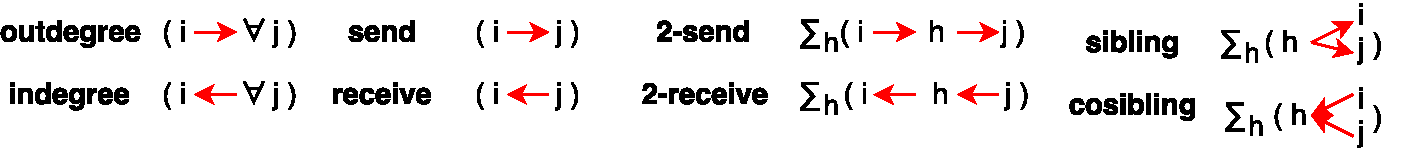
\includegraphics[height= 2cm, trim= 0cm 0cm 14cm 0cm, clip=true]{figures/netstats.pdf}\\ \vspace{-.5cm}
		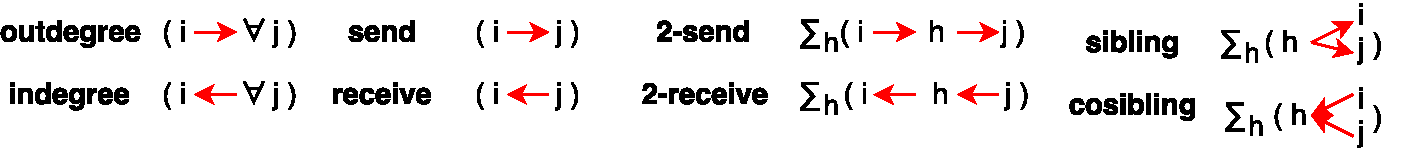
\includegraphics[height= 2cm,, trim= 10cm 0cm 0cm 0cm, clip=true]{figures/netstats.pdf}
	 \end{figure}	

\end{frame}

\begin{frame}{Conditioning features on recency}


\begin{itemize}
\item Network features conditioned on degree of recency
\item Partition the past 384 hours (=16 days) into 3 sub-intervals
	\begin{equation*}
	[t-384h,t) = [t-384h, t-96h) \cup [t-96h, t-24h)\cup [t-24h, t),
	\end{equation*}
\item $\boldsymbol{x}^{(c)}_{t, l}(i, j)$ is the network statistics at time $t$, for interaction pattern $c$
\end{itemize}
\centering
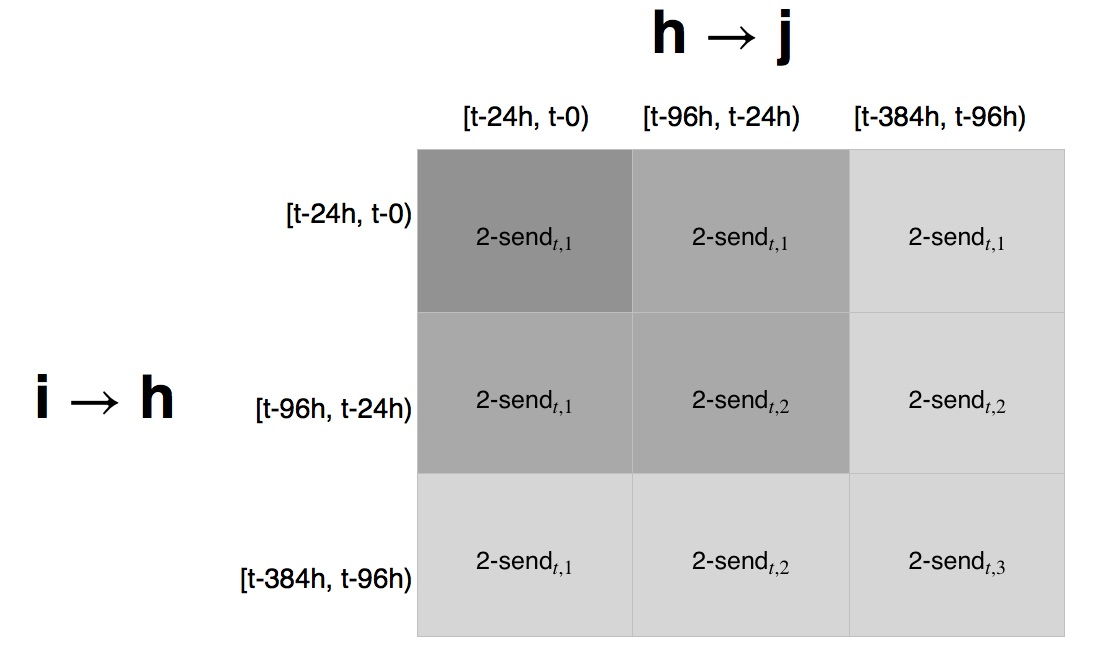
\includegraphics[scale=.2]{./figures/triadtable}

\end{frame}

\begin{frame}{Tie generating process: receivers}
		\begin{itemize}
		\item [1.] For each sender $i \in \{1,...,A\}$ and receiver $j \in \{1,...,A\}$ ($i \neq j$), calculate the stochastic indensity between $i$ and $j$:
	%	\footnotesize
			\begin{equation*}\lambda^{(d)}_{ij}=\sum\limits_{c=1}^{C} p^{(d)}_c
		\cdot  \mbox{exp}\Big\{ \boldsymbol{b}^{(c)T}\boldsymbol{x}^{(c)}_{t^{(d-1)}}(i, j)\Big\},	\end{equation*}\normalsize
		which is a mixture of contents and network effects.\\ \vspace{0.4cm}
		\item[2.] For each sender $i \in \{1,...,A\}$, choose a binary vector $J^{(d)}_i$ of length $(A-1)$, by applying Gibbs measure (Fellows and Handcock, 2017) 
	%	\footnotesize
		%\mbox{log}\big(\text{I}( \sum_{j \in \mathcal{A}_{\backslash i}} J^{(d)}_{ij} > 0 )\big) + 
		\begin{equation*} \text{P}(J_i^{(d)}) \propto \exp\Big\{ \sum_{j \in \mathcal{A}_{\backslash i}} (\delta+\mbox{log}(\lambda_{ij}^{(d)}))J_{ij}^{(d)} \Big\},
		\end{equation*}
		\normalsize
		where $\delta$ is a real-valued intercept controlling the recipient size\\ \vspace{0.1cm}
 \begin{figure}
 	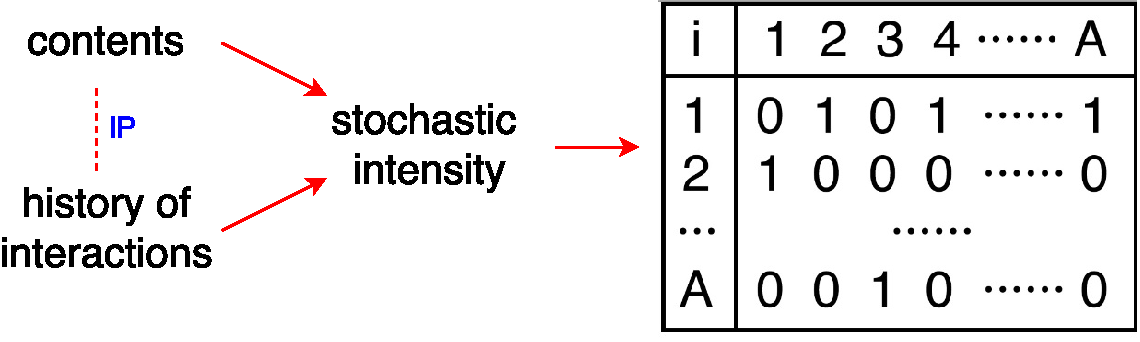
\includegraphics[width=0.4\textwidth]{figures/edge.pdf}
 \end{figure}	
	\end{itemize}
	\end{frame}
\begin{frame}{Tie generating process: sender and time}
\begin{itemize}
		\item [3.] For each sender $i \in \{1,...,A\}$, generate the time increments for document $d$
	%	\footnotesize
		\begin{equation*}
		\Delta T^{(d)}_{i{J_i}} \sim \mbox{Exponential}(\eta\lambda_{i{J_i}}^{(d)}),
		\end{equation*}\normalsize
		where $\eta$ is the positive real-valued parameter for time-increments and \footnotesize$\lambda^{(d)}_{iJ_i}= \sum\limits_{c=1}^{C} p^{(d)}_c\cdot\mbox{exp}\Big\{\textcolor{black}{\frac{1}{|J_i|}\sum\limits_{j \in J_i} \boldsymbol{b}^{(c)T}\boldsymbol{x}^{(c)}_{t^{(d-1)}}(i, j)}\Big\}\quad$\normalsize is the updated sender-specific stochastic intensity given the receivers.\vspace{0.4cm}
		\item[4.] Set the observed sender, receivers and timestamp simultaneously:
		%\footnotesize
			\begin{equation*}
		\begin{aligned}
		&i^{(d)} = i_{\mbox{min}(\Delta T^{(d)}_{i{J_i}})} \\
		&J^{(d)} = J_{i^{(d)}}\\
		&t^{(d)} = t^{(d-1)}+\mbox{min}(\Delta T^{(d)}_{i{J_i}})\\
		\end{aligned}
		\end{equation*}
		\normalsize
\end{itemize}
 %\begin{figure}
 %	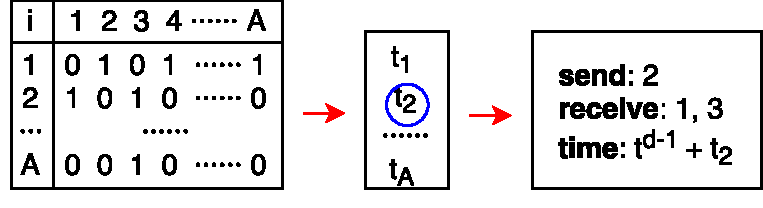
\includegraphics[width=0.57\textwidth]{figures/tie.pdf}
 %\end{figure}	
\end{frame}

\begin{frame}{Joint generating process}

	\begin{figure}
		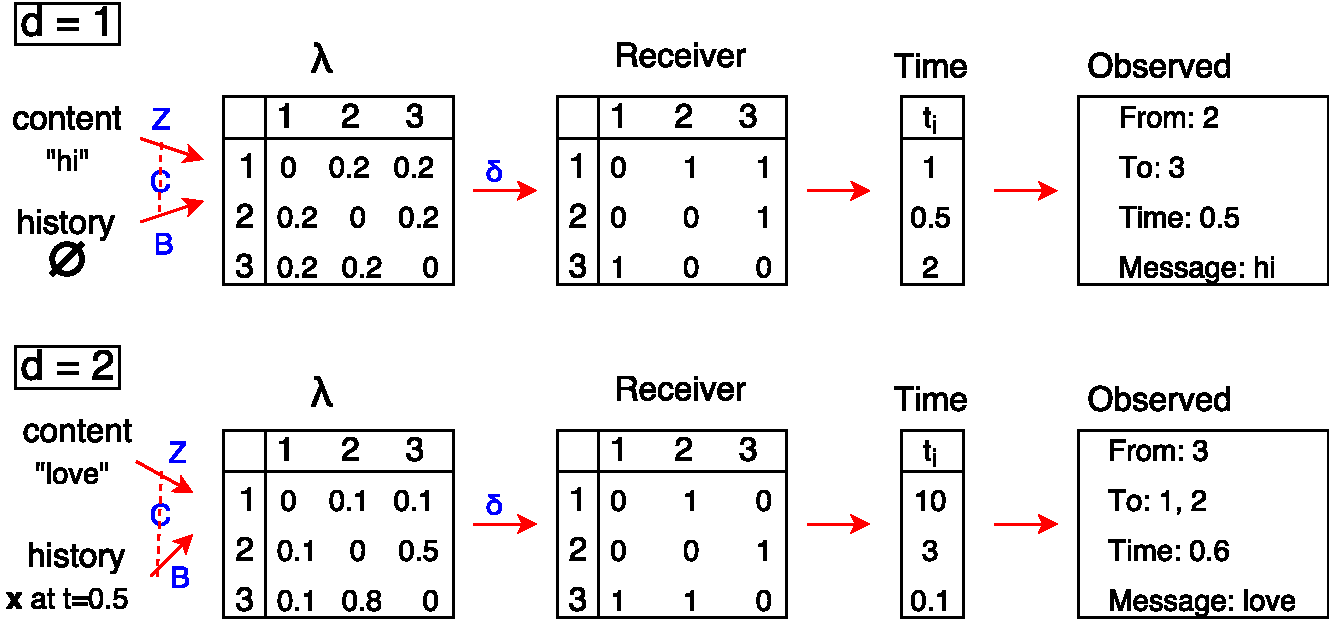
\includegraphics[width=0.9\textwidth]{figures/summary.pdf}
	\end{figure}	\vspace{0.1cm}

\end{frame}


\begin{frame}{Inference}

\begin{itemize}
\item Take a Bayesian approach to inference
\item $\mathcal{B}$, $\delta$, and $\eta$ interpreted at fixed $\mathcal{Z}$ and  $\mathcal{C}$
\end{itemize}
  	\begin{center}
  		\scalebox{.9}{	 
 	 \begin{minipage}{1\linewidth}\begin{algorithm}[H]
\SetAlgoLined
	 	\caption{MCMC}
	 	Set initial values $\mathcal{Z}^{(0)}, \mathcal{C}^{(0)}, $ and $(\mathcal{B}^{(0)}, \delta^{(0)},  \eta^{(0)})$\\
	 	\For{o=1 to O}{
	 				Sample the \textcolor{blue}{latent receivers} $J^{(d)}_{ij}$ via Gibbs sampling\\
	 				Sample the \textcolor{blue}{topic assignments} $\mathcal{Z}$ via Gibbs sampling\\
	 			Sample the \textcolor{blue}{interaction pattern assignments} $\mathcal{C}$ via Gibbs sampling\\
	 		 				Sample the \textcolor{blue}{network effect parameters} $\mathcal{B}$  via Metropolis-Hastings \\
	 			Sample the \textcolor{blue}{receiver size parameter} $\delta$ via Metropolis-Hastings\\
	 			Sample the \textcolor{blue}{timing parameter} $\eta$ via Metropolis-Hastings
	 	}
	 \end{algorithm}
	\end{minipage}}
	 	\end{center}
\end{frame}


\begin{frame} \frametitle{Getting it Right: jointly testing math and code}

Geweke (2004) proposed a test for Bayesian posterior samplers \vspace{.2cm}
\begin{itemize}
\item {\em Forward samples}: 
\begin{enumerate}
\item Draw parameters from prior
\item Draw data conditional on parameters
\item Repeat
\end{enumerate} \vspace{.2cm}
\item {\em Backward samples}: 
\begin{enumerate}
\item Start with a forward sample of data
\item Run inference on data
\item Generate new data conditioned on inferred parameters
\item Run inference on new data
\item Repeat
\end{enumerate} \vspace{.2cm}
\item Forward samples and backward samples should match
\end{itemize}


\end{frame}

\begin{frame} \frametitle{GiR results}
\begin{center}
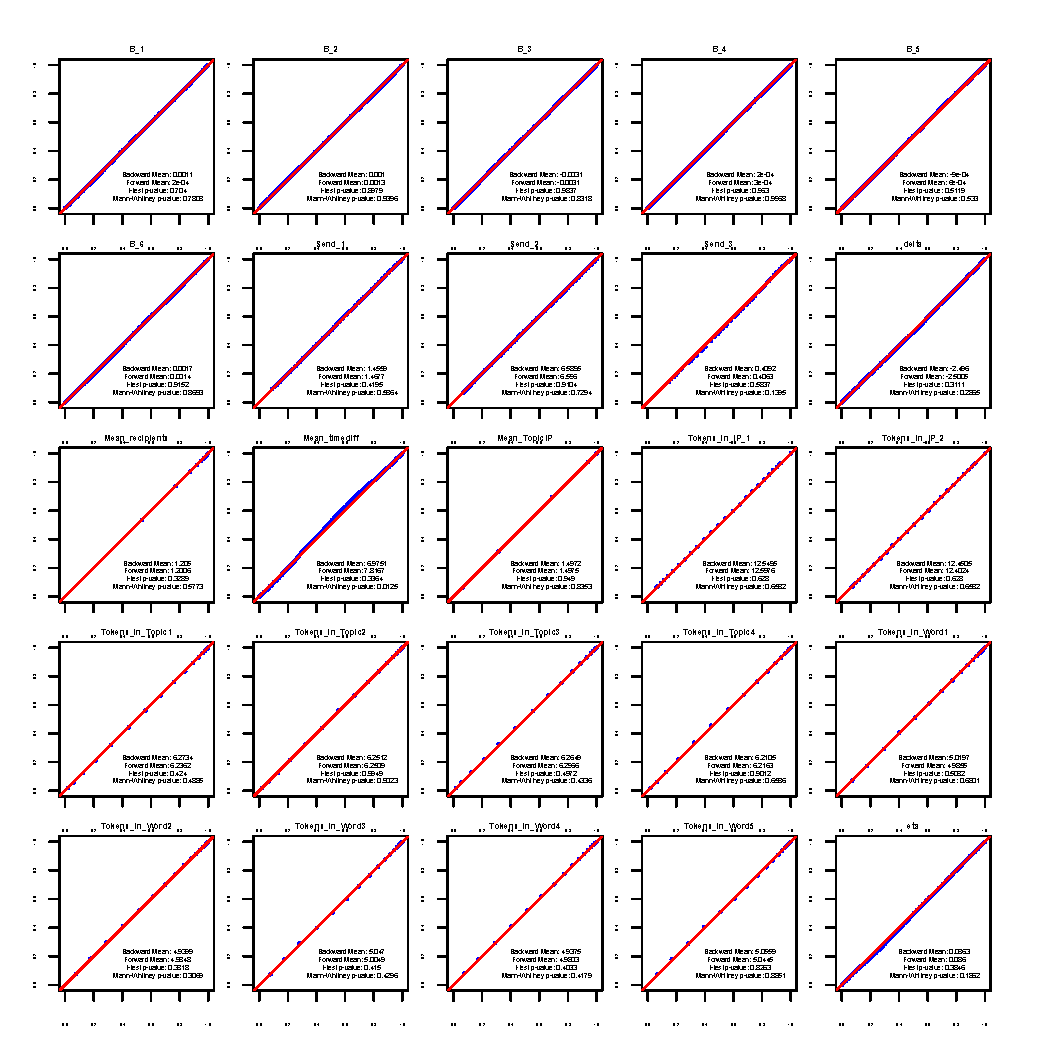
\includegraphics[width=0.78\textwidth]{./figures/GiReta} 
\end{center}
\end{frame}



\begin{frame}{Dare County, NC email data}
\begin{center} 
\includegraphics[width=0.75\textwidth]{figures/Dare.png}
\end{center}
 \begin{itemize}
 \item $D = 2210$ emails
\item  $A = 27$ county government managers
\item  $W = 2907$ unique words
\item  covering 3 month period (September 1 - November 30) in 2012
\item Hurricane Sandy passed by NC: October 26 - October 30
 \end{itemize}
\end{frame}


\begin{frame}{Theoretical considerations}
\large
\begin{itemize}
\item Personal/friendship topics exhibit reciprocity and transitivity \vspace{.4cm}
\item Professional communications avoid loops  \vspace{.4cm}
\item Sandy communications represent pattern breakdowns
\end{itemize}

\end{frame}



\begin{frame}{Exploratory data analysis: Dare County}
	\begin{minipage}{0.85\linewidth}
	 	 \begin{figure}
	 	 	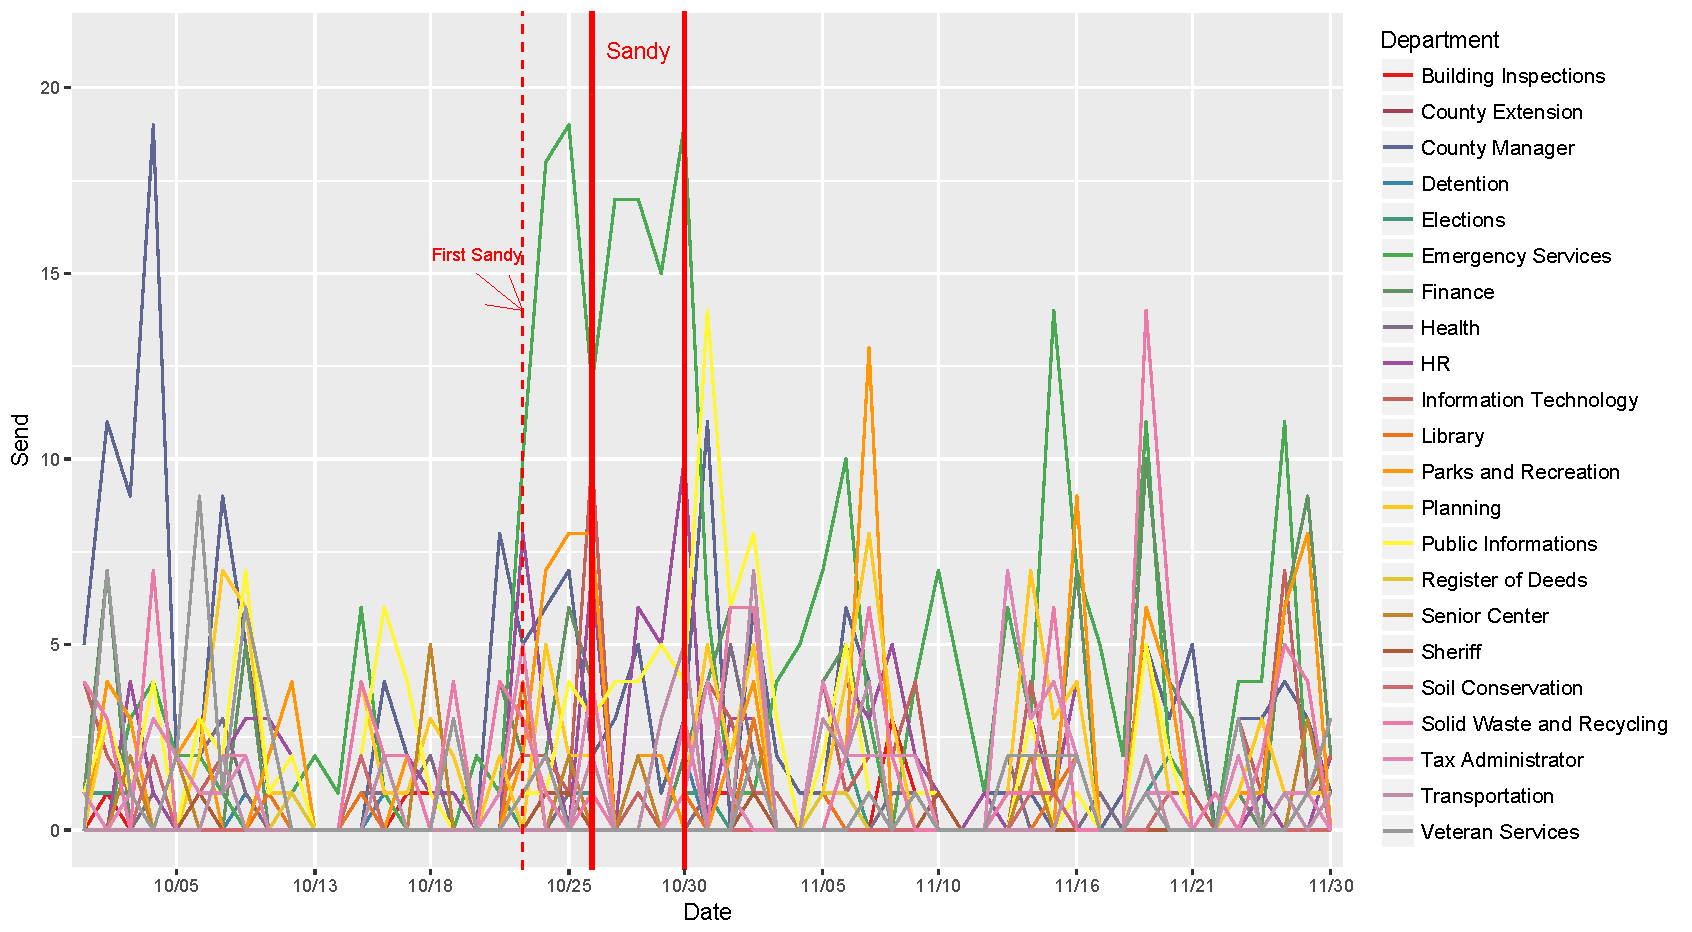
\includegraphics[width=0.5\textwidth, trim = 0cm 0cm 6cm 0cm, clip=true]{figures/DareSend.pdf}	 	
	 	 	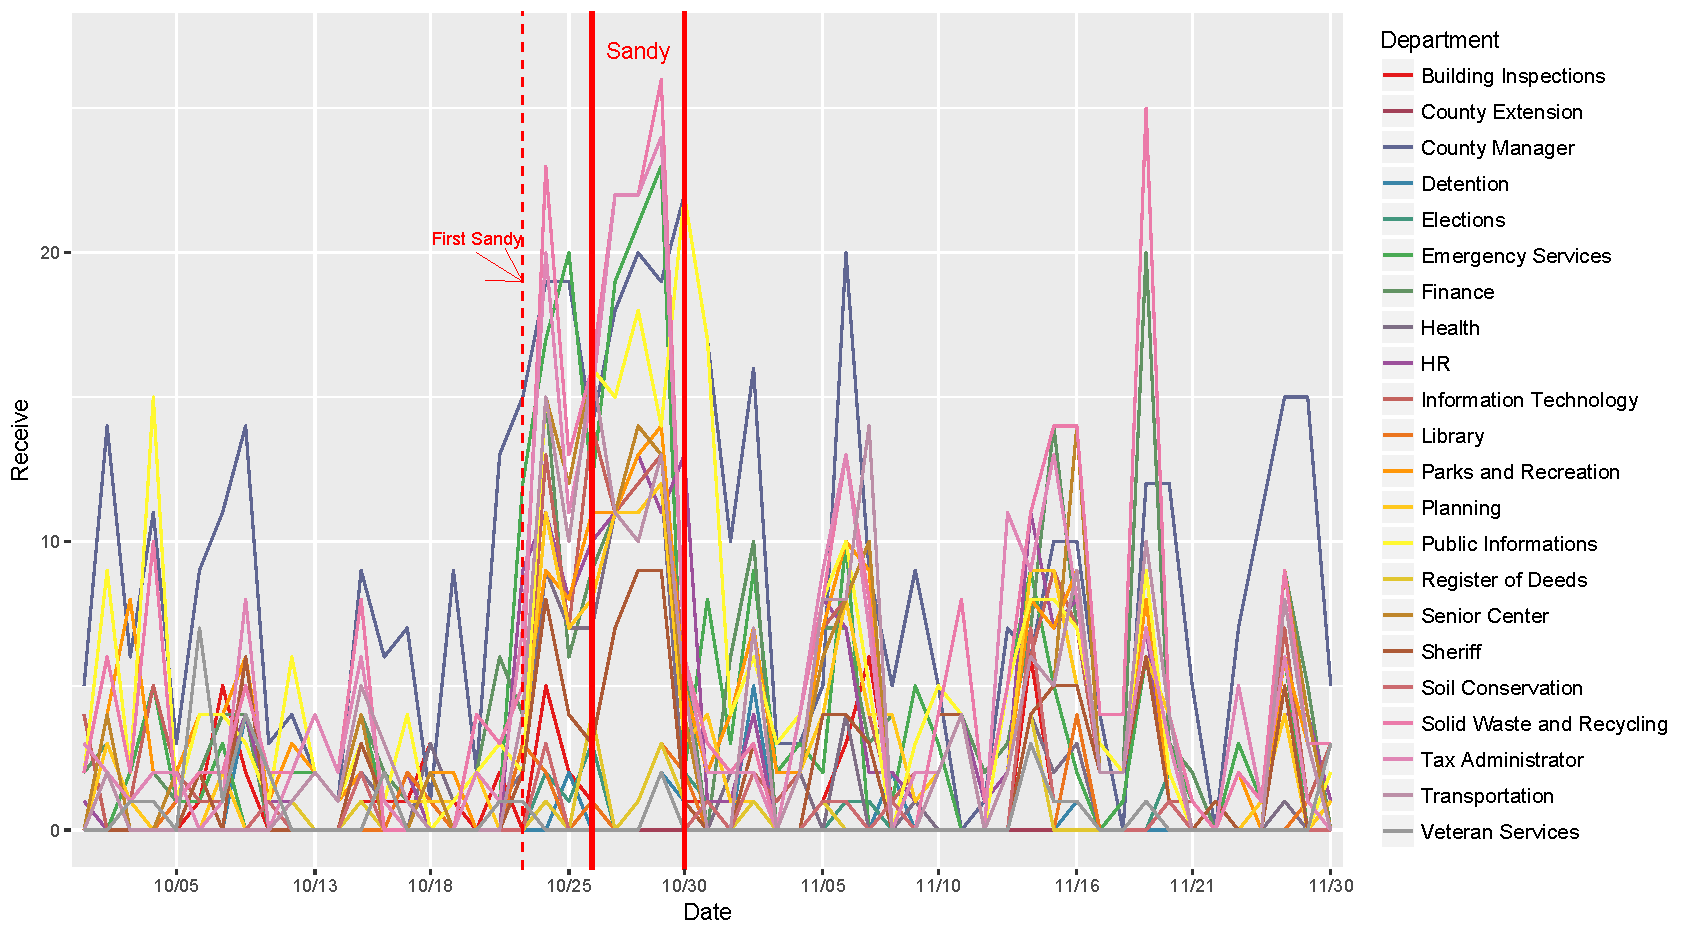
\includegraphics[width=0.5\textwidth, trim = 0cm 0cm 6cm 0cm, clip=true]{figures/DareReceive.pdf}
	 	 \end{figure}	\vspace{-.5cm}
	 \begin{figure}
	 %	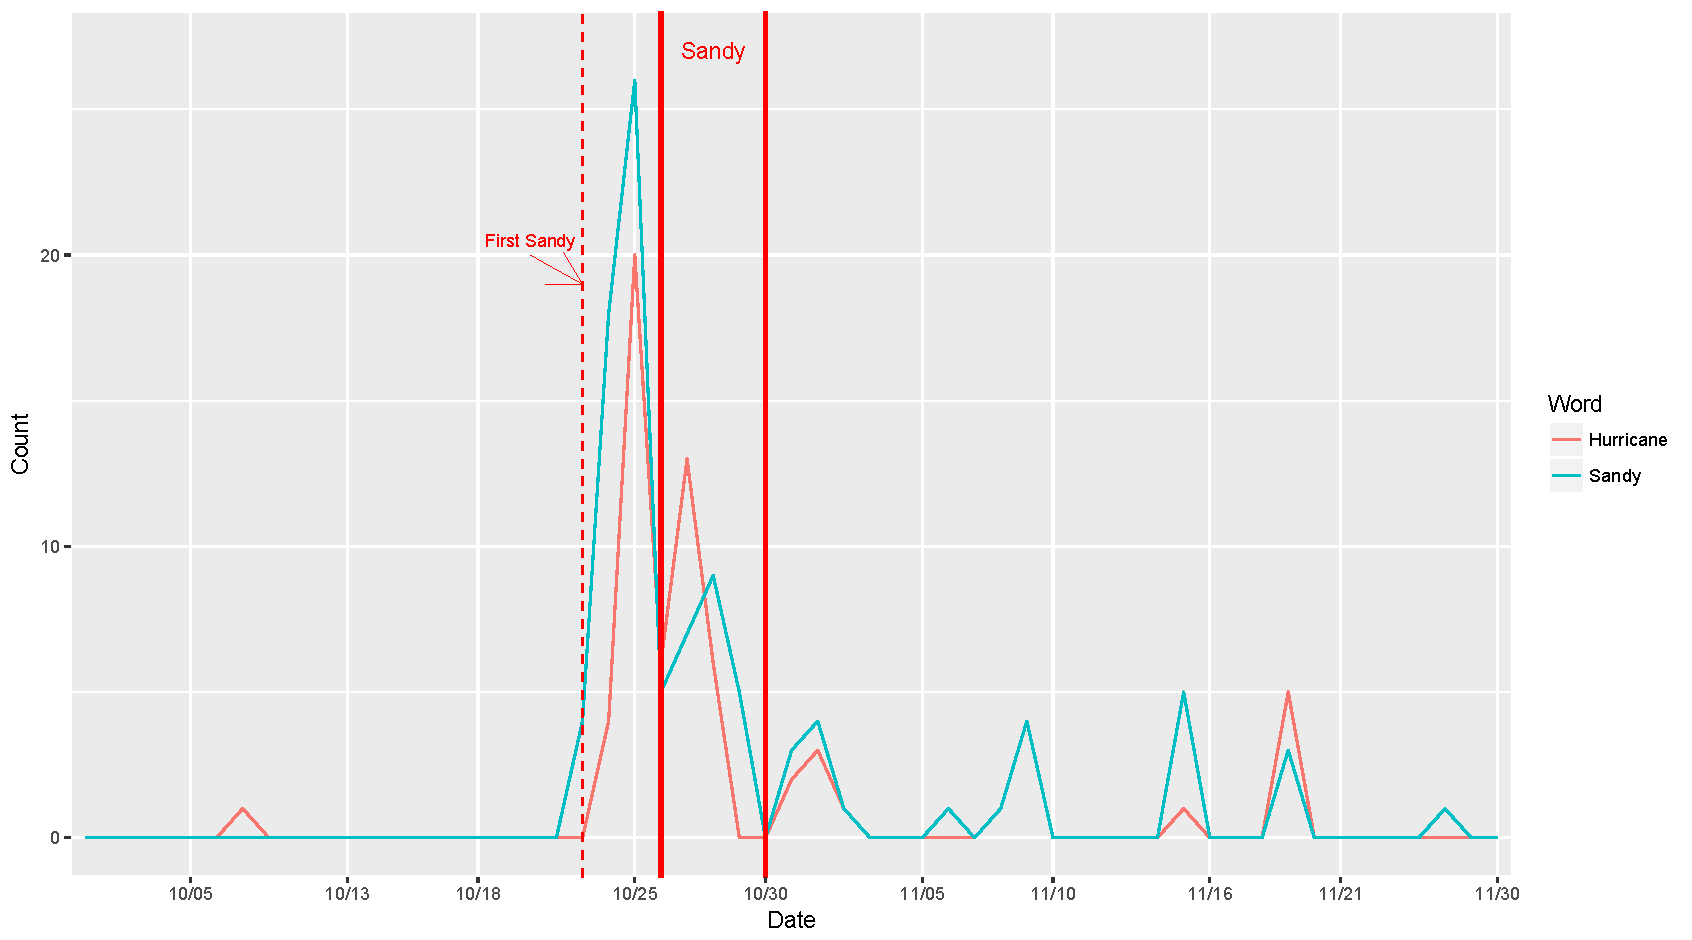
\includegraphics[width=0.5\textwidth]{Wordplot.pdf}	 
	 		 	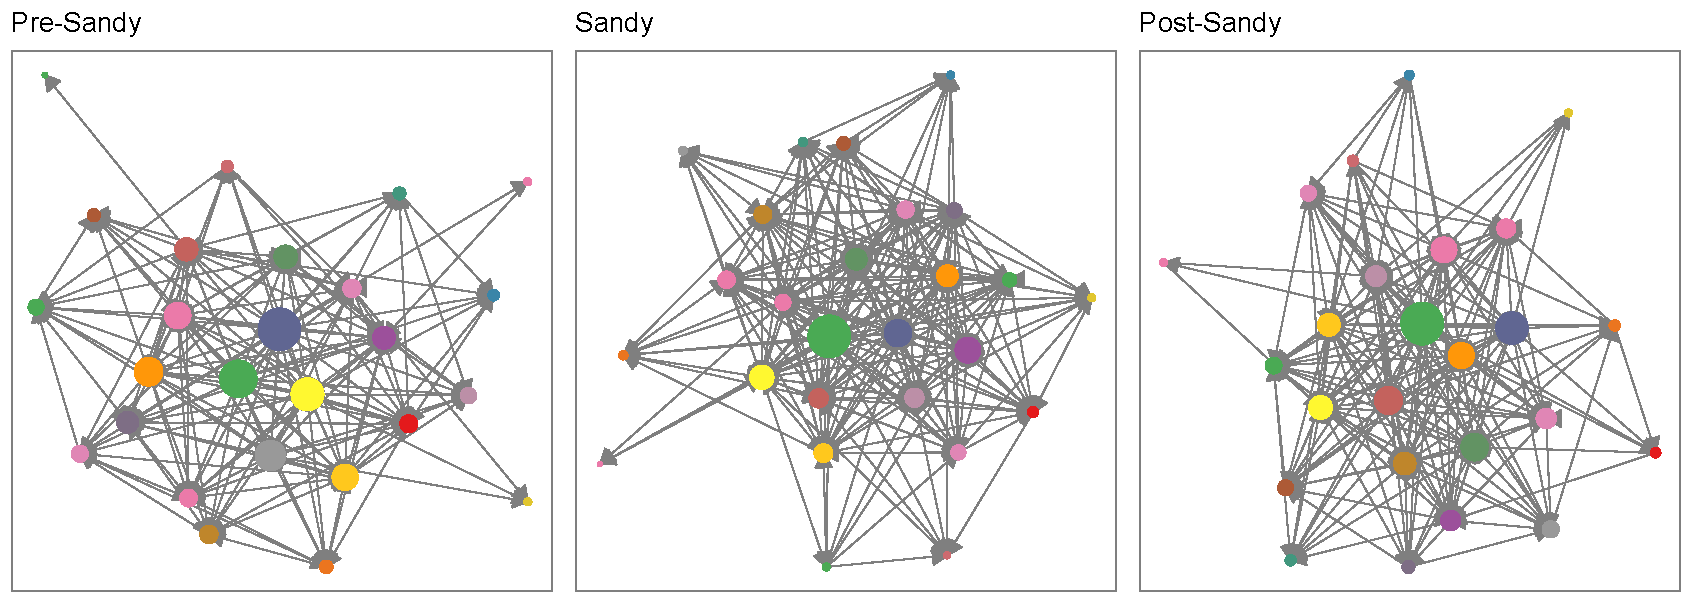
\includegraphics[width=1\textwidth]{figures/DareNetwork.pdf}
	 		 		 \end{figure}	
\end{minipage}
\begin{minipage}{0.13\linewidth}
		 \begin{figure}
	 		 		 	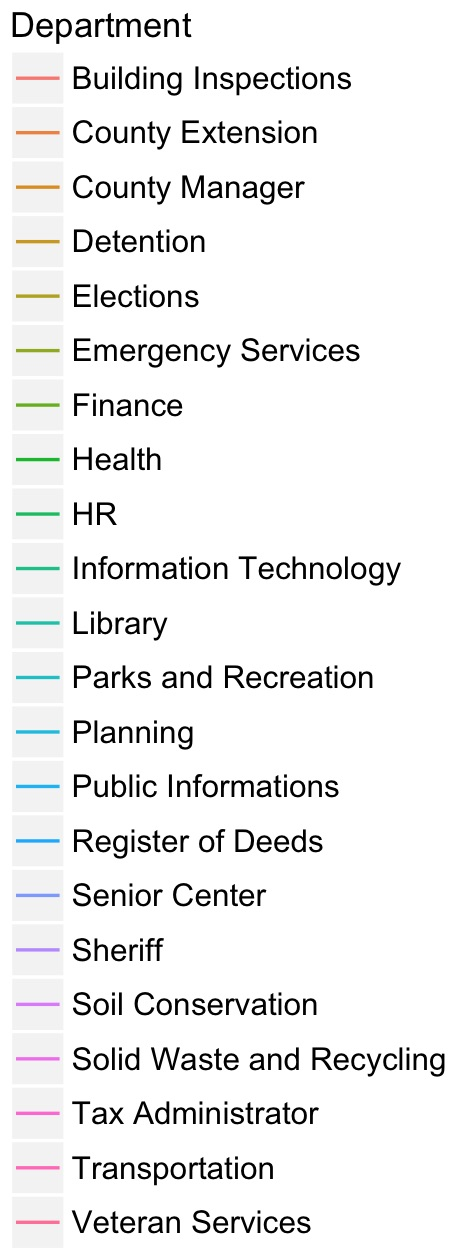
\includegraphics[width=1.25\textwidth]{figures/Dept2.jpg}
	 \end{figure}	
	\end{minipage}
\end{frame}



 \begin{frame}{IPTM result: topics (IP=1)}
 \centering
 	 $C=2$, $K=25$ and $O= 100$
  	\scalebox{0.75}{	 	\begin{tabular}{ |c||c|c|c|c|c|}  
  			\hline
  			\textbf{IP} & \textbf{1} &  \textbf{1} & \textbf{1}  &\textbf{1} &\textbf{1}   \\ \hline\hline
  			\textbf{Topic} & \textbf{23} (0.055)&   \textbf{18} (0.054) &\textbf{11} (0.048)&\textbf{20} (0.033) &\textbf{8} (0.032)  \\ \hline\hline
  			\textbf{Word} 
  		& change & will &  \cellcolor{blue!25} sandy & time & services\\
  		& order & \cellcolor{blue!25}  winds &  munis & hours & public \\
  		& manager &  location & \cellcolor{blue!25} hurricane& monday & white\\
  		&\cellcolor{blue!25} storm & \cellcolor{blue!25} beach &  position & leave & director \\
  		& \cellcolor{blue!25}emergency &  \cellcolor{blue!25} hydrant & monday &employees & fyi\\
  		&\cellcolor{blue!25} coastal & \cellcolor{blue!25} water & point & timesheets &tim \\
  		& statute & relocation &  power& \cellcolor{blue!25} storm & \cellcolor{blue!25} update \\
  		& \cellcolor{blue!25}evacuation & mirlo & update & employee & \cellcolor{blue!25} status\\
  		&\cellcolor{blue!25} track &  road & \cellcolor{blue!25} storm& tomorrow &board \\
  		& couple & high & hey & work & approval\\
  		& changes & moving & release& regular &wanted\\
  		& well & gas & weeks & period &rec\\
  		& concerns & \cellcolor{blue!25}  forecast & weekend & comp & adult\\
  		& things & saturday & working&sheets &older\\
  		& consistent & project & month& vacation & today\\
  		&\cellcolor{blue!25} boat &  \cellcolor{blue!25} outer & problems&administrative &\cellcolor{blue!25} storm  \\
  		 & misdemeanor & map & \cellcolor{blue!25} strong& operation & reminder\\
  		 & program &airport & \cellcolor{blue!25} impacts & timesheet &called\\
  		 & \cellcolor{blue!25} system &called &  three & personnel & sep\\
  		 & powerpoint &  \cellcolor{blue!25} banks & ncdot & will &charlotte \\
  			\hline            				
  		\end{tabular}}
\end{frame}


 \begin{frame}{IPTM result: topics (IP=2)}
 \centering
 	 $C=2$, $K=25$ and $O= 100$
  	\scalebox{0.75}{	 	\begin{tabular}{ |c||c|c|c|c|c|}  
  			\hline
  			\textbf{Topic} &   \textbf{21} (0.057)& \textbf{12} (0.037) &\textbf{14} (0.037) &\textbf{4} (0.035)&\textbf{10} (0.026) \\ \hline\hline
  			\textbf{Word}
  			& library & marshall & will&board & survey\\
  			& best & collins &center&meeting & request\\
  			& start & drive &day& property &call \\
  			& web & manteo & office&planning & sure\\
  			& place & phone & great&will & people\\
  			& visit &box & manager&notice &emergency \\
  			& albermarle & fax &assistance&  january & thought\\
  			& east & resources & problem& review & seafood\\
  			&regional & director & lot&commissioners & mail\\
  			&system & human & call&list & grant\\
  			&voice &phr &  currently&thoughts & ncacc \\
  			& librarian &policy &september& amendment &community\\
  			& learning & time &early&  members &check \\
  			& discovery & october &parking& dot & rodanthe\\
  			& manteo & hire & received&budget & district\\
  			& expressed & will & monday& building & complete\\
  			& views & offices & baum&inspections &option \\
  			& box & approved &questions& night &best\\
  			& conversion & hour & year&text & residents\\
  			& director &told&today& copy &talk\\  			\hline            				
  		\end{tabular}}
\end{frame}

\begin{frame}{IPTM result: example email}
\begin{itemize}
	\item From: 11 (Public Infromations)\\
	\item To: 4 (Emergency Services) and 18 (Detention)\\	 
	\item At: 25 Oct 2012 19:14:47\\
	\item Content:
\textcolor{blue}{ will will storm good \textcolor{black}{sure} sandy morning morning morning morning send change plan hurricane wanted copy base afternoon keep description description saturday saturday saturday saturday touch touch release signature plans prior ready duration submitted eoc running exactly activation activation released mind joint jis pasted \textcolor{black}{activate}}
	\end{itemize}
\end{frame}


\begin{frame}{IPTM result: dynamic network effects, Dare County}
\begin{changemargin}{-1cm}{-1cm}
	\begin{figure}
		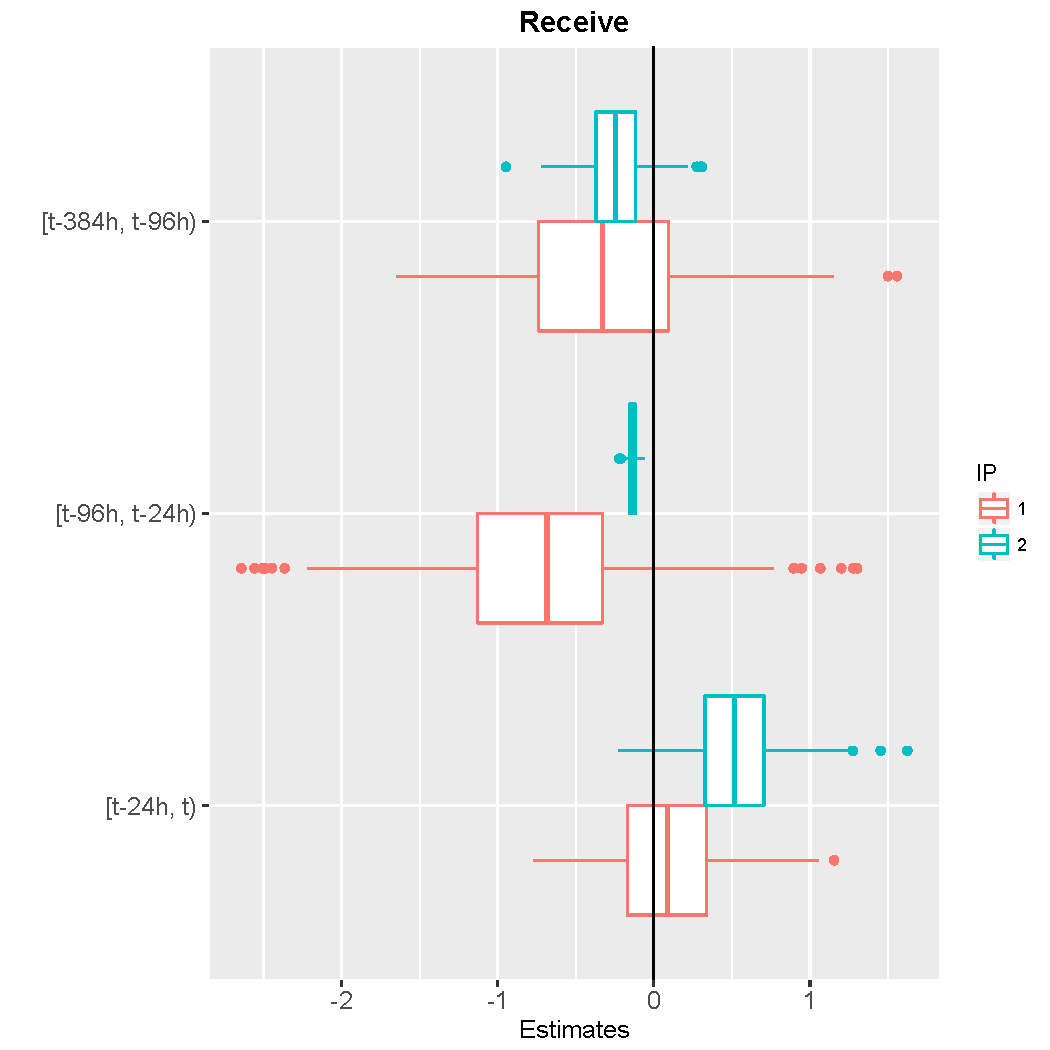
\includegraphics[width=.55\textwidth]{figures/receive.pdf} 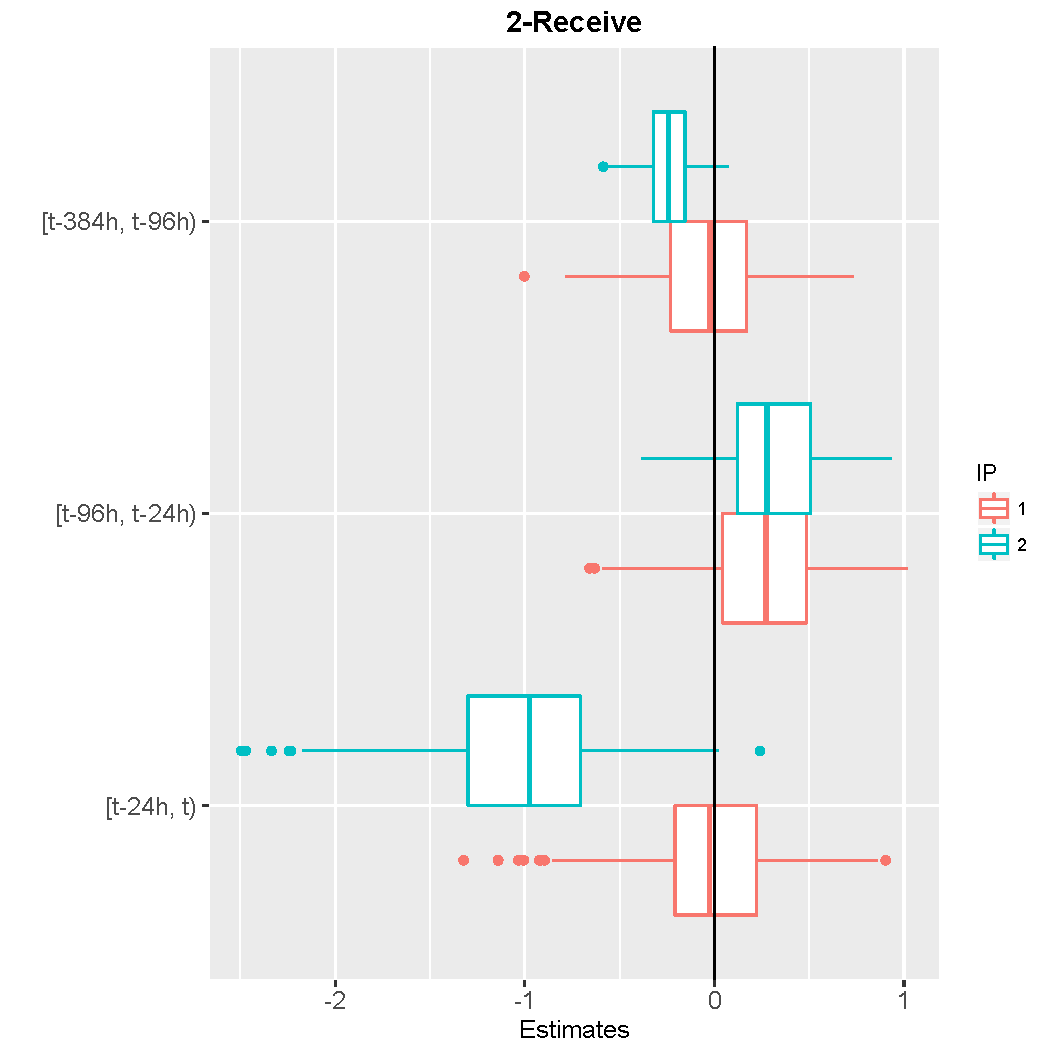
\includegraphics[width=.55\textwidth]{figures/2receive.pdf}
			\end{figure}
	\end{changemargin}
\end{frame}


\begin{frame} \frametitle{Model fit evaluation}
\begin{itemize}
\item Forecast topics, ties, and timing of next document
\item Compare to one or more models that can generate same predictions
\end{itemize}
 	\begin{center}
\scalebox{.8}{
 \begin{minipage}{1\linewidth}
\begin{algorithm}[H]
	\SetAlgoLined
	\caption{Predicting tie data for the next document}
	
	Input
	\begin{enumerate}
	\item $O$, number of outer iterations of inference from which to generate predictions
	\item $d$, the last document to use in inference
	\item $R$, the number of iterations to sample predicted data within each outer iteration
	\end{enumerate}
	Run burnin iterations\\
	\For{o=1 to O}{
		run an outer iteration of inference on documents $1$ through $d$\\
		initialize values for $i^{(d+1)}$, $J^{(d+1)}$, $t^{(d+1)}$, and $\mathcal{Z}^{d+1}$ \\
		\For{r=1 to R}{
		sample  $i^{(d+1)}$, $J^{(d+1)}$, and $t^{(d+1)}$ conditional on $\mathcal{Z}^{d+1}$, via the generative process \\
		sample $\mathcal{Z}^{d+1}$ via Equation 24
		}
		store $i^{(d+1)}$, $J^{(d+1)}$, $t^{(d+1)}$, and $\mathcal{Z}^{d+1}$
	}
\end{algorithm}
\end{minipage}
}
\end{center}
\end{frame}


\begin{frame} \frametitle{Model fit evaluation}
\begin{center}
	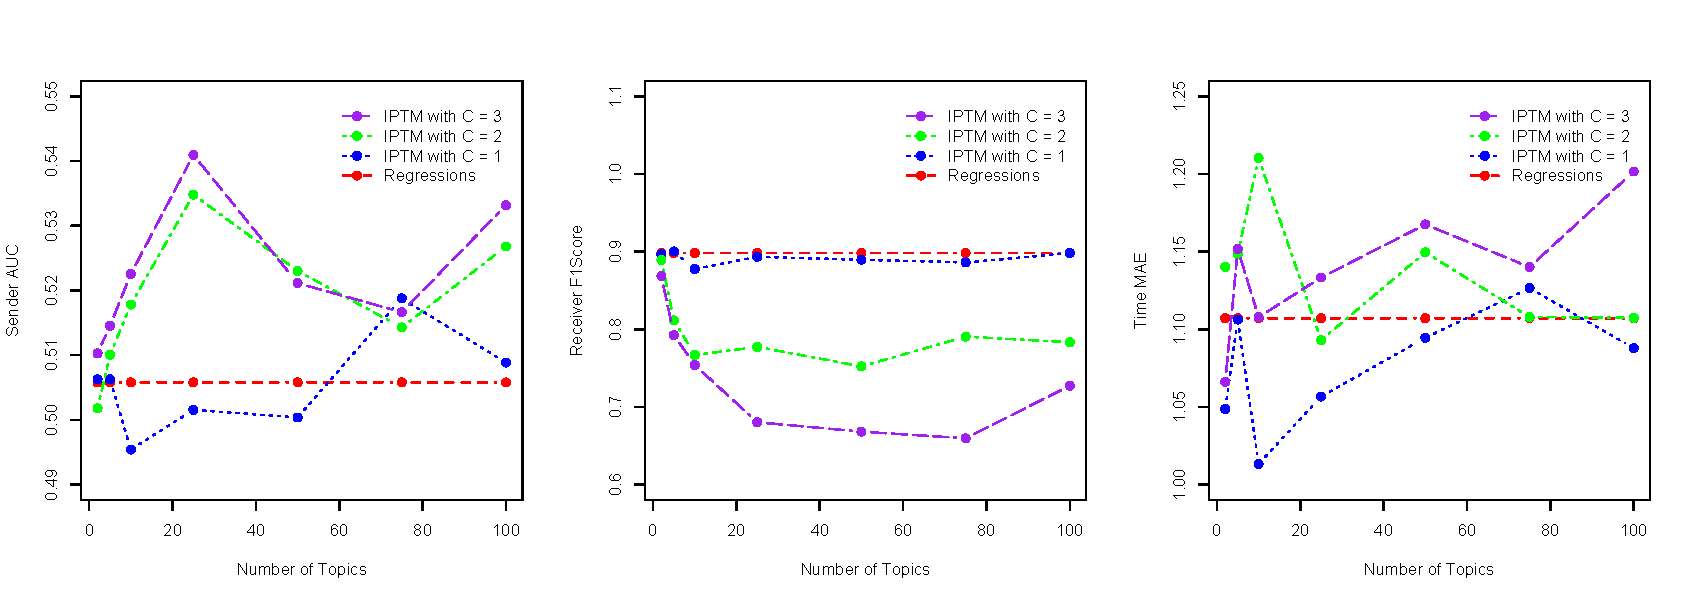
\includegraphics[width=1\textwidth]{figures/Dare_PPE_22.pdf}
	\end{center}
\begin{itemize}
	\item Area under the ROC curve (AUC) for sender, F1-score for Receivers, and Mean Absolute Error (MAE) for timing
	\item $C=1$ loses the connection between ties and text
	\item Lack of fit in predicting receivers and timing
	\item Further modfications to improve model fits
\end{itemize}
\end{frame}


\begin{frame}{Conclusion}
 \bni
 \item Joint modeling of ties (sender, receiver, time) and contents
 	\vspace{0.4cm}
 \item Contribution in distribution for non-empty multicast
 	\vspace{0.4cm}
 \item Many potential applications in political science
 	\vspace{0.4cm}
 	\item Developement of R package `IPTM'
 \ei
\end{frame}




\end{document}